
\documentclass[12pt]{article}
\usepackage[a4paper, margin=.30in]{geometry}
\usepackage{graphicx ,
            wrapfig,
            xcolor, 
            enumerate,
            amsmath,
			fontenc,
			tcolorbox,circuitikz
            }

\newcommand\headerMe[2]{\noindent{}#1\hfill#2}
\renewcommand{\thesection}{\Roman{section}}

\author{Zakaria HAOUZAN}
\date{\today}

\begin{document}
% headers --------------
\headerMe{Matière : Physique-Chimie}{Professeur : Zakaria HAOUZAN}\\
\headerMe{Unité : Electricité }{Établissement : Lycée SKHOR qualifiant}\\
\headerMe{Niveau : 2BAC-SM-PC}{Heure : 6H}\\

% ------Content ________
\begin{center}

    \Large{Leçon $N^{\circ} 8 $: \color{red} Circuit RLC série }
\end{center}

%\begin{wrapfigure}[10]{r}{0.5\textwidth}
%    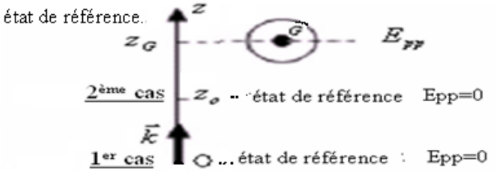
\includegraphics[width=0.5\textwidth]{./img/img00.png}
%\end{wrapfigure}

\section{La Bobine : }
\subsection{Définition : }
Le circuit RLC est constitué d'un condensateur initiallement chargé monté en série avec une
résistance R et une bobine

\section{Oscillations libres dans un circuit RLC série.}
\subsection{Décharge d’un condensateur dans une bobine.}
\subsubsection{Etude expérimentale.}
\begin{wrapfigure}{r}{0.3\textwidth}
	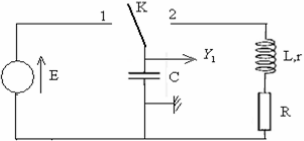
\includegraphics[width=0.3\textwidth]{./img/Rlc_00.png}
\end{wrapfigure}


On réalise le montage suivant :

On place l'interrupteur K à la position (1) une durée suffisante pour que le condensateur soit chargé puis le bascule à
la position 2 tout en visualisant à la voie y1 sur l'écran d'un oscilloscope la tension aux bornes du condensateur .

On obtient ainsi un circuit RLC en série dans lequel la charge emmagasinée dans le condensateur oscille entre ses armatures car le
condensateur se décharge et se charge régulièrement mais grâce à l'existence de la résistance dans le circuit , la charge du
condensateur diminue de même que la tension entre ses bornes :on dit que les oscillations sont amorties .

Et comme le circuit RLC ne comporte pas de générateur : \textbf{les oscillations sont dites libres et amorties }.
(l'amortissement est due au fait qu'une partie de l'énergie électrique se perd sous forme de chaleur au niveau de la résistance
du circuit par effet Joule).
\subsubsection{Les régime d'amortissement : }
Selon la valeur de la résistance on distingue trois régimes:



\textbf{Le régime périodique }: Si la résistance totale du circuit est nulle les oscillations sont libres et non amorties

\begin{center}
	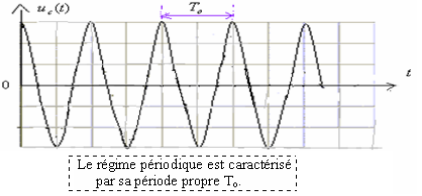
\includegraphics[width=0.4\textwidth]{./img/Rlc_01.png}
\end{center}

\textbf{Le régime pseudopériodique } : Si la résistance totale du circuit est faible les oscillations sont libres et amorties et leur
amplitude diminue jusqu'à ce qu'il s'annule. ( c'est l'état de l'amortissement faible).

\begin{center}
	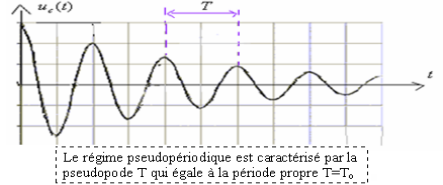
\includegraphics[width=0.4\textwidth]{./img/Rlc_02.png}
\end{center}


\textbf{Le régime apériodique: }Si la résistance totale du circuit est grande, les oscillations disparaissent car l'amortissement est
fort, le condensateur perd sa charge sans oscillations et on distingue dans ce cas trois régimes:

\begin{itemize}
	\item Le régime sous critique : la tension aux bornes du condensateur effectue une seule oscillation avant de s'annuler.

	\item Le régime critique : la tension aux bornes du condensateur s'annule sans oscillations.
	\item Le régime surcritique : la tension aux bornes du condensateur dure un temps très long pour s'annule sans oscillations.
\end{itemize}


\begin{center}
	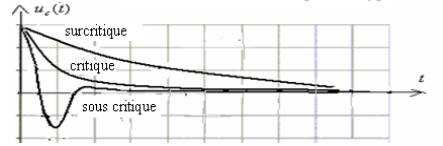
\includegraphics[width=0.4\textwidth]{./img/Rlc_03.png}
\end{center}

\subsubsection{Equation différentielle d'un circuit RLC en série : }


On considère le montage suivant dans lequel le condensateur est initialement chargé.

En appliquant la loi d'additivité des tensions on a: $u_C + u_R + u_L = 0$ 

donc $$\frac{d^u_C}{dt^2} + \frac{R_t}{L}.\frac{du_C}{dt} + \frac{1}{LC}.u_C = 0$$ avec $R_t=R + r$ et C'est l'équation différentielle que vérifie la tension aux bornes du condensateur dans un circuit RLC en série. 

Le terme $\frac{R_t}{L}.\frac{du_C}{dt}$ résulte de l'amortissement (par son annulation l'amortissement disparait).


\section{Oscillations non amorties dans un circuit idéal LC :}
\subsection{Etude expérimentale.}

On considère le montage expérimental suivant constitué d'un condensateur de capacité C initialement chargé et d'une bobine
idéale d'inductance L et de résistance nulle r=0.(ce qui est difficile de réaliser pratiquement car quelque soit la bobine , sa
résistance est non nulle , donc c'est un circuit idéal)


\subsection{Equation différentielle : }

En appliquant la loi d'additivité des tensions: $u_L + u_C = 0$ donc  $$\frac{d^2u_C}{dt^2} + \frac{1}{LC}.u_C = 0$$

C'est l'équation différentielle que vérifie la tension aux bornes du condensateur dans un circuit idéal LC.

\subsection{Solution de l'équation  différentielle : }

La solution de l'équation différentielle: $\frac{d^2u_C}{dt^2} + \frac{1}{LC}.u_C = 0$
est une fonction sinusoïdale de la forme : 
$$u_C(t) = U_m.cos(\frac{2\pi}{T_0}.t + \phi) $$

\begin{itemize}
	\item $u_C (t)$: tension aux bornes du condensateur. en (V)
	\item $U_m$ :amplitude des oscillations :(c'est l'élongation maximale ) en (V)
	\item $\phi$ : la phase du mouvement à l'instant t=0. en (rad).
	\item $T_0$ : la période propre des oscillations en (s)
\end{itemize}

\subsection{Expression de la période propre : }

Or la solution de l'équation différentielle: $\frac{d^2u_C}{dt^2} + \frac{1}{LC}.u_C = 0$ est $u_C(t) = U_m.cos(\frac{2\pi}{T_0}.t + \phi) $

En remplaçant dans l'équation différentielle on Trouve que $T_0 = 2\pi.\sqrt{LC}$

\subsection{Utilisation de l'équation de dimension pour Déterminer l'Unité de $T_0$}

On a $T_0 = 2\pi.\sqrt{LC}$ donc $[T_0] = ([L][C])^2$

d'après la relation : $i = C\frac{du_C}{dt}$ et $u_L = L\frac{di}{dt}$ donc $[T_0] = [t]$

\subsection{Expression de l'intensité du courant et de la charge dans le circuit idéal LC : }

L'expression de la charge du condensateur en fonction du temps est : $q(t) = C.u_C(t)$ avec

$u_C(t) = U_m.cos(\frac{2\pi}{T_0}.t + \phi)$

qu'on peut écrire  :$$q(t) = q_m.cos(\frac{2.\pi}{T_0}.t + \phi)$$ avec $q_m = C.U_m$

L'expression de l'intensité du courant: 

$i(t) = \frac{dq}{dt} = -q_m.\frac{2.\pi}{T_0} . sin(\frac{2.\pi}{T_0}.t + \phi) = q_m.\frac{2\pi}{T_0}.cos(\frac{2\pi}{T_0}.t + \phi + \frac{\pi}{2})$  car $-sin(\alpha) = cos(\alpha + \frac{\pi}{2})$

qu'on peut écrire : $$i(t) = I_m.cos(\frac{2\pi}{T_0}.t + \phi + \frac{\pi}{2} )$$ avec $I_m = q_m. \frac{2\pi}{T_0}$ 

Pour déterminer la valeur de $\phi $ on utilise les conditions initiales qui sont $u_C(t) = E$ à $t = 0$

donc en remplaçant dans $u_C(t = 0) = E$ elle devient $cos(\phi) = \frac{E}{E} =1$ donc $\phi = 0$

donc: $$q(t) = q_m.cos(\frac{2\pi}{T_0}t) et i(t) = I_m.Cos(\frac{2\pi}{T_0} + \frac{\pi}{2})$$ 

q(t) et: i(t). sont en quadrature de phase.(lorsque l'une est maximale ou bien minimale l'autre s'annule.)

\begin{center}
\begin{tabular}{ |c| c| c|c|c|c|c| }
	\hline
	t   & 0 & $\frac{T_0}{4}$ & $\frac{T_0}{2}$ &$\frac{3.T_0}{4}$&$T_0$ \\\hline 
	q(t)&+ $q_m$& 0               &$-q_m$           &$0$ & +$q_m$ \\\hline 
	i(t)&0      & $-I_m$    &0           &$+I_m$ & 0 \\\hline 
\end{tabular}
\end{center}


\begin{center}
	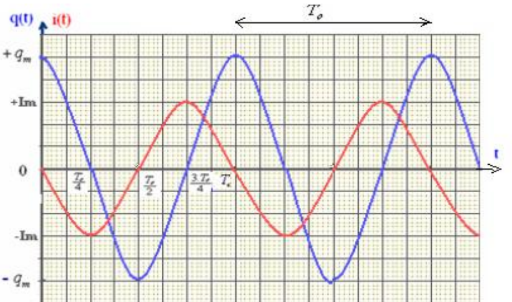
\includegraphics[width=0.4\textwidth]{./img/Rlc_05.png}
\end{center}

\section{Transfert d'énergie entre la bobine et le condensateur : }

\subsection{Energie du circuit LC : }
\subsubsection{Expression de l'énergie totale d’un circuit LC: }
L'énergie totale d'un dipôle LC est la somme de l'énergie électrique emmagasinée dans le condensateur et de
l'énergie magnétique emmagasinée dans la bobine.

$$\xi = \frac{1}{2}.\frac{q^2}{C} + \frac{1}{2}.L.i^2$$

On a
\begin{itemize}
	\item $u(t) = U_m.cos(\frac{2\pi}{T_0}.t + \phi)$
	\item $q(t) = C.u(t) = q_m.cos(\frac{2\pi}{T_0}.t + \phi)$
	\item $i(t) = \frac{dq}{dt} = -q_m.\frac{2\pi}{T_0}sin(\frac{2\pi}{T_0}.t + \phi)$
	\item $T_0^2 = 4\pi^2 .L.C$

\end{itemize}

Alors $$\xi = \frac{q_m^2}{2.C}$$

avec $I_m = q_m.\frac{2.\pi}{T_0}$ donc $q_m = \frac{I_m.T_0}{2\pi}$

donc $q_m =LCI_m^2$

$$\xi_t = \frac{1}{2}.\frac{q_m^2}{C} = \frac{1}{2}.L.I_m^2$$


et On a $q_m = C.E$ $$\xi = \frac{1}{2}.CE^2$$

donc:l'énergie totale du circuit LC est constante.

\subsubsection{Courbes de variation des énergies d'un circuit idéal LC:}

La période T de l'échange énergétique entre la bobine et le condensateur est égale à la moitié de la période propre To.
Au cours des oscillations non amorties, l'énergie électrique emmagasinée dans le condensateur se transforme en énergie magnétique emmagasinée dans la bobine et inversement.


\begin{center}
	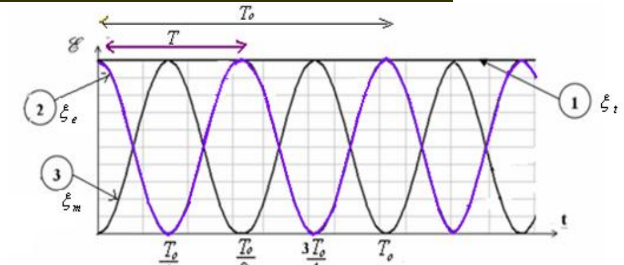
\includegraphics[width=0.4\textwidth]{./img/Rlc_06.png}
\end{center}

\subsubsection{Détermination de l'équation différentielle par étude énergétique: }

L'énergie totale d'un dipôle LC est constante $\xi_t = Cst$ donc $\frac{d\xi}{dt} = 0$ avec $\xi_t = \xi_e  + \xi_m$

$$\frac{d^2u_C}{dt^2} + \frac{1}{L.C}.u_C = 0$$

C'est l'équation différentielle que vérifie la tension aux bornes du condensateur dans un circuit idéal LC.

\subsection{Energie du circuit RLC en série : }

L'énergie totale d'un dipôle RLC est : $\xi_t = \frac{1}{2}.L.i^2 + \frac{1}{2}.\frac{q^2}{c}$

En appliquant la loi d'additivité des tensions On a : $u_R + u_C + u_L = 0$

donc $$L.\frac{di}{dt} + u_C = -R_t.i$$ avec $ R_t =R + r $

d'autre part on a : $\frac{\xi_t}{dt} = L.i\frac{di}{dt} + \frac{q}{c}.\frac{dq}{dt}= i.(L.\frac{di}{dt} + \frac{q}{c} ) = -R_t.i^2$

donc $\frac{d\xi_t}{dt} = -R_t.i^2  < 0$ donc l'énergie totale du circuit RLC est décroissante.

L'énergie totale du circuit RLC décroit en fonction du temps et les oscillations sont amorties à cause de la perte de
l'énergie électrique par effet joule au niveau de la résistance.

\begin{center}
	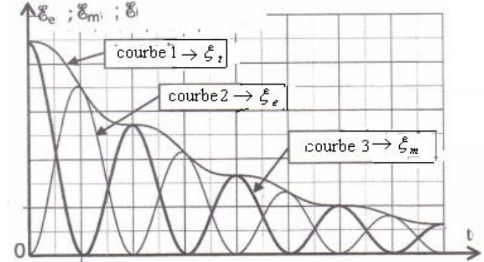
\includegraphics[width=0.4\textwidth]{./img/Rlc_07.png}
\end{center}


\section{Entretien des oscillations : }
Pour entretenir les oscillations on doit utiliser un générateur d'entretient pour récompenser l'énergie perdue par effet Joule à
chaque oscillation.

\begin{center}
	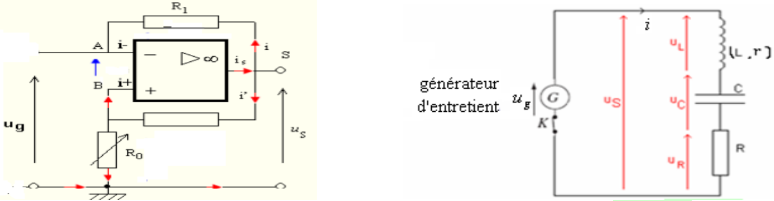
\includegraphics[width=0.5\textwidth]{./img/Rlc_08.png}
\end{center}




La tension aux bornes du générateur d'entretient est proportionnelle à l'intensité du courant $u_g = R_0.i$ avec $R_0 = R+r$

Ce générateur se comporte comme une résistance négative.
En appliquant la loi d'additivité des tensions on a: $u_g = u_R + u_C + u_L$

$$LC.\frac{d^2u_C}{dt^2} + u_C = 0$$

C'est l'équation différentielle que vérifie la tension aux bornes du condensateur dans un circuit idéal LC.donc les oscillations
sont entretenues et l'amplitude devient constante.

\begin{center}
	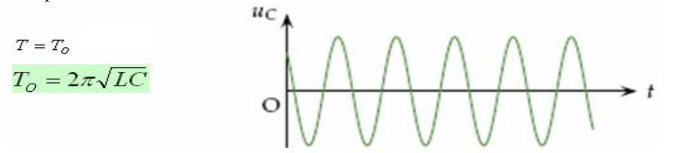
\includegraphics[width=0.4\textwidth]{./img/Rlc_09.png}
\end{center}




%wfg---------------------------------------------------------------sf 
%\begin{center}
   %\begin{tabular}{ |c|c|c|c|c|c|c| }
      %\hline
      %km & hm & dam & \bf{m} & dm & cm & mm \\
      %\hline
        %&   &    &  &   &   & \\
%\hline
%\end{tabular}
%On place un seul nombre dans chaque case.
%\end{center}
%\begin{center}
   %\begin{tabular}{ |c|c|c|c|c|c|c| }
      %\hline
      %$km^2$ & $hm^2$ & $dam^2$ & \bf{$m^2$} & $dm^2$ & $cm^2$ & $mm^2$ \\
      %\hline
        %&   &    &  &   &   & \\
%\hline
%\end{tabular}
%\end{center}


\end{document}

